\documentclass[12pt]{beamer}

% Theme & Colors
\usetheme{Madrid} % Try: Berlin, Copenhagen, CambridgeUS, Warsaw...
\usecolortheme{dolphin} % Try: seahorse, crane, beaver...

% Encoding & Fonts
\usepackage[utf8]{inputenc}
\usepackage[T1]{fontenc}
\usepackage{lmodern} % Better font
\usepackage{luatexja}
\usepackage{luatexja-fontspec}
\usepackage{amsmath,amssymb,mathtools,ascmac,amsthm,amscd,tikz-cd}
\usetikzlibrary{arrows.meta,calc,quotes,angles}
\setmainjfont{Noto Sans CJK JP}
% Title Information
\newcommand{\circnum}[2][]{%
  \tikz[baseline=(n.base)] \node (n) [circnum,#1]{#2};%
}
\title[]{チェバの定理\\メネラウスの定理}
\date{\today}

\begin{document}
% Title Page
\begin{frame}
  \titlepage
\end{frame}

% Outline
\begin{frame}{}
  \tableofcontents
\end{frame}

% Section 1
\section{チェバの定理 (Ceva's theorem)}
\begin{frame}{}
  \begin{block}{チェバの定理 (Ceva's theorem)}
		\triangle ABCの内部(または外部)にある$X$と3頂点を結んだ直線$AX, BX, CX$
		がそれぞれの対辺と点{\color{blue}$P,Q,R$}で交わるとき,
\[\frac{AR}{RB}\cdot\frac{BP}{PC}\cdot\frac{CQ}{QA} = 1.\]
  \end{block}
	\begin{center}
	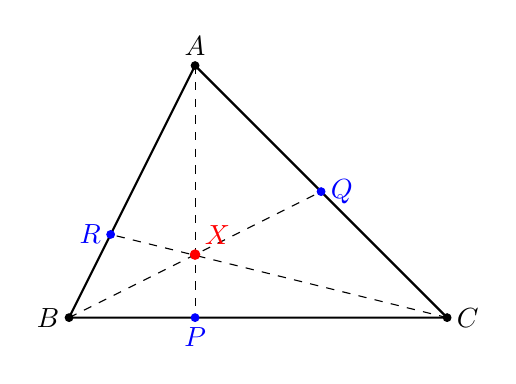
\begin{tikzpicture}[scale=1.6]
  % Define the vertices
  \coordinate (B) at (0,0);
  \coordinate (C) at (3,0);
  \coordinate (A) at (1,2);
  \coordinate (P) at (1,0);
  \coordinate (Q) at (2,1);
  \coordinate (R) at (0.33,0.66);
  % Draw the triangle
  \draw[thick] (A)--(B)--(C)--cycle;

  % Compute centroid G = (A+B+C)/3
  \coordinate (X) at (1,0.5);

  % Draw medians
  \draw[dashed] (A)--(P);
  \draw[dashed] (B)--(Q);
  \draw[dashed] (C)--(R);
  % Mark the points
  \fill (A) circle (1pt) node[above] {$A$};
  \fill (B) circle (1pt) node[left] {$B$};
  \fill (C) circle (1pt) node[right] {$C$};
	\fill[blue] (P) circle (1pt) node[below] {$P$};
	\fill[blue] (Q) circle (1pt) node[right] {$Q$};
	\fill[blue] (R) circle (1pt) node[left] {$R$};
  \fill[red] (X) circle (1.2pt) node[above right] {$X$};
\end{tikzpicture}
\end{center}
\end{frame}

\begin{frame}{}
	\begin{block}{補題.}
	1辺を共有する2つの三角形\triangle ABCと\triangle DBCに対して,
	\[\frac{\triangle ABC}{\triangle DBC} = \frac{AP}{DP}.\]
	\end{block}
\begin{center}
	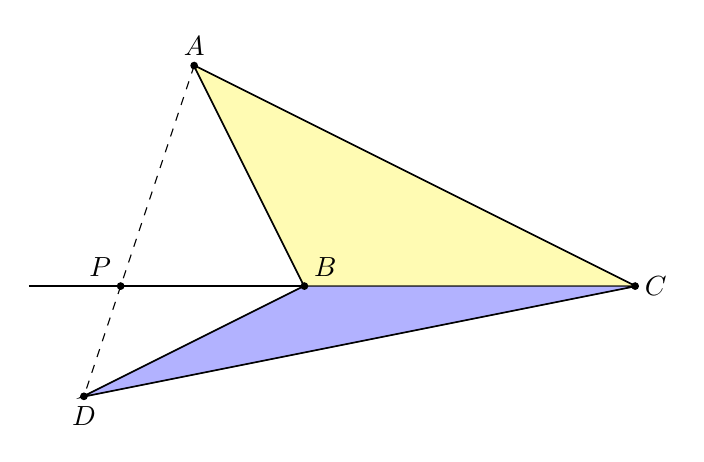
\begin{tikzpicture}[scale=1.4]
  % Define the vertices
  \coordinate (B) at (0,0);
  \coordinate (B') at (-2.5,0);
  \coordinate (C) at (3,0);
  \coordinate (A) at (-1,2);
	\coordinate (D) at (-2,-1);
	\coordinate (P) at (-5/3,0);
  % Draw the triangle
  \draw[thick] (C)--(A)--(B);
  \draw[thick] (B)--(D)--(C);
  \draw[thick] (B')--(C);
  \draw[dashed] (A)--(D);

	\draw[fill=yellow!30] (A)--(B)--(C)--cycle;
	\draw[fill=blue!30] (D)--(B)--(C)--cycle;

  % Mark the points
  \fill (A) circle (1pt) node[above] {$A$};
  \fill (B) circle (1pt) node[above right] {$B$};
  \fill (C) circle (1pt) node[right] {$C$};
  \fill (D) circle (1pt) node[below] {$D$};
  \fill (P) circle (1pt) node[above left] {$P$};
\end{tikzpicture}
\end{center}
\end{frame}
\begin{frame}{チェバの定理の証明}
	\begin{center}
	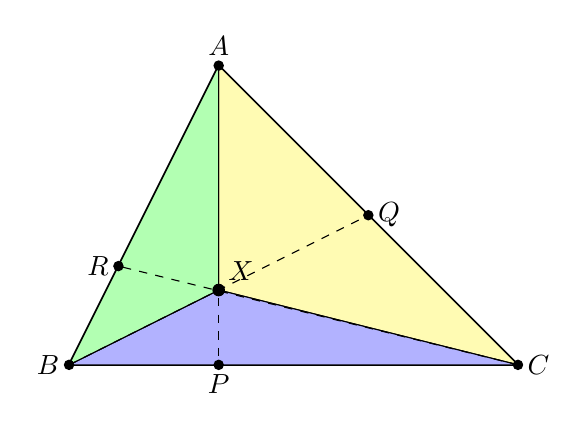
\begin{tikzpicture}[scale=1.9]
  % Define the vertices
  \coordinate (B) at (0,0);
  \coordinate (C) at (3,0);
  \coordinate (A) at (1,2);
  \coordinate (P) at (1,0);
  \coordinate (Q) at (2,1);
  \coordinate (R) at (0.33,0.66);
  \coordinate (X) at (1,0.5);
  % Draw the triangle
  \draw[thick] (A)--(B)--(C)--cycle;

	\draw[fill=yellow!30] (A)--(X)--(C)--cycle;
	\draw[fill=blue!30] (B)--(X)--(C)--cycle;
	\draw[fill=green!30] (A)--(X)--(B)--cycle;

  % Compute centroid G = (A+B+C)/3

  % Draw medians
  \draw[dashed] (A)--(P);
  \draw[dashed] (B)--(Q);
  \draw[dashed] (C)--(R);
  % Mark the points
  \fill (A) circle (1pt) node[above] {$A$};
  \fill (B) circle (1pt) node[left] {$B$};
  \fill (C) circle (1pt) node[right] {$C$};
	\fill (P) circle (1pt) node[below] {$P$};
	\fill (Q) circle (1pt) node[right] {$Q$};
	\fill (R) circle (1pt) node[left] {$R$};
  \fill (X) circle (1.2pt) node[above right] {$X$};
\end{tikzpicture}
\end{center}
補題から,
\begin{align*}
	\frac{AR}{RB}\cdot\frac{BP}{PC}\cdot\frac{CQ}{QA}  &= \frac{\triangle XAC}{\triangle XBC}\cdot\frac{\triangle XAB}{\triangle XAC}\cdot \frac{\triangle XBC}{\triangle XAB} = 1.
\end{align*}
		\hfill \blacksquare
\end{frame}

\begin{frame}{$X$が外部にある場合}
	\begin{center}
		\begin{tikzpicture}[scale=1.5]
  % Define the vertices
  \coordinate (B) at (0,0);
  \coordinate (B') at (-1.5,-3);
  \coordinate (C) at (3,0);
  \coordinate (C') at (4.5,-1.5);
  \coordinate (A) at (1,2);
  \coordinate (P) at (1.8,0);
  \coordinate (Q) at (4,-1);
  \coordinate (R) at (-1,-2);
  \coordinate (X) at (2,-0.5);
  % Draw the triangle
  \draw[thick] (A)--(B)--(C)--cycle;
  \draw[thick] (B')--(B);
  \draw[thick] (C')--(C);

  % Draw medians
  \draw[dashed] (A)--(X);
  \draw[dashed] (B)--(Q);
  \draw[dashed] (C)--(R);
  % Mark the points
  \fill (A) circle (1pt) node[above] {$A$};
  \fill (B) circle (1pt) node[left] {$B$};
  \fill (C) circle (1pt) node[right] {$C$};
	\fill[blue] (P) circle (1pt) node[above left] {$P$};
	\fill[blue] (Q) circle (1pt) node[right] {$Q$};
	\fill[blue] (R) circle (1pt) node[left] {$R$};
  \fill[red] (X) circle (1.2pt) node[above right] {$X$};
\end{tikzpicture}
	\end{center}
\end{frame}

% Section 2
\section{メネラウスの定理 (Menelaus's theorem)}
\begin{frame}{}
  \begin{block}{メネラウスの定理 (Menelaus's theorem)}
		\triangle ABCの頂点を通らない直線$\ell$が直線$BC, CA, AB$とそれぞれ{\color{blue}$P,Q,R$}で交わるとき,次が成り立つ.
		\[\frac{AR}{RB}\cdot\frac{BP}{PC}\cdot\frac{CQ}{QA} = 1.\]
  \end{block}
	\begin{center}
	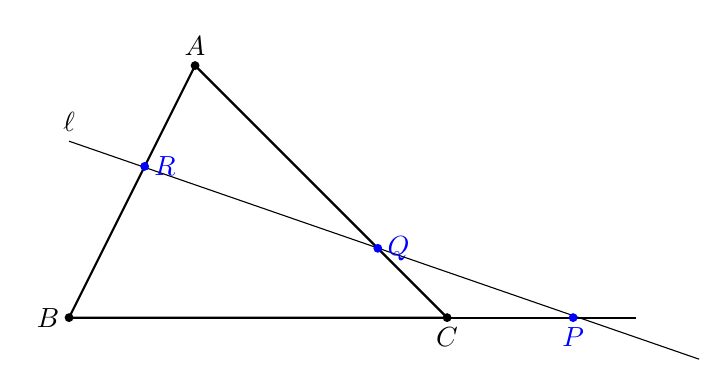
\begin{tikzpicture}[scale=1.6]
  % Define the vertices
  \coordinate (B) at (0,0);
  \coordinate (C) at (3,0);
	\coordinate (C') at (4.5,0);
  \coordinate (A) at (1,2);
  \coordinate (P) at (4,0);
  \coordinate (P') at (5,-0.33);
  \coordinate (Q) at (2.45, 0.55);
  \coordinate (R) at (0.6,1.2);
  \coordinate (R') at (0,1.4);
  % Draw the triangle
  \draw[thick] (A)--(B)--(C)--cycle;
  \draw[thick] (B)--(C');
  % Draw medians
	\draw[] (P')--(R') node[above] {$\ell$};
  % Mark the points
  \fill (A) circle (1pt) node[above] {$A$};
  \fill (B) circle (1pt) node[left] {$B$};
  \fill (C) circle (1pt) node[below] {$C$};
	\fill[blue] (P) circle (1pt) node[below] {$P$};
	\fill[blue] (Q) circle (1pt) node[right] {$Q$};
	\fill[blue] (R) circle (1pt) node[right] {$R$};
\end{tikzpicture}
\end{center}
\end{frame}

\begin{frame}{証明.}
	$\ell$に平行で$C$を通る直線$\ell '$を引き,$AB$との交点を$D$とする.
\begin{center}
	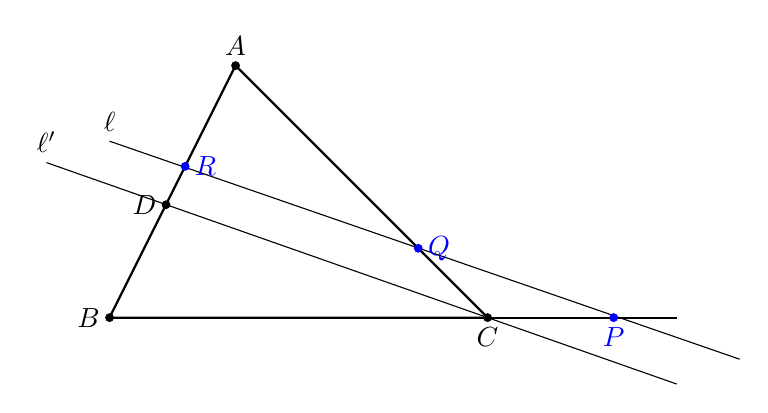
\begin{tikzpicture}[scale=1.6]
  % Define the vertices
  \coordinate (B) at (0,0);
  \coordinate (C) at (3,0);
	\coordinate (C') at (4.5,0);
  \coordinate (A) at (1,2);
  \coordinate (P) at (4,0);
  \coordinate (P') at (5,-0.33);
  \coordinate (Q) at (2.45, 0.55);
  \coordinate (R) at (0.6,1.2);
  \coordinate (R') at (0,1.4);
  \coordinate (E) at (-0.5,1.23);
  \coordinate (F) at (4.5,-0.527);
  \coordinate (D) at (0.448,0.896);
  % Draw the triangle
  \draw[thick] (A)--(B)--(C)--cycle;
  \draw[thick] (B)--(C');
  % Draw medians
	\draw[] (P')--(R') node[above] {$\ell$};
	\draw[] (F)--(E) node[above] {$\ell '$};
  % Mark the points
  \fill (A) circle (1pt) node[above] {$A$};
  \fill (B) circle (1pt) node[left] {$B$};
  \fill (C) circle (1pt) node[below] {$C$};
  \fill (D) circle (1pt) node[left] {$D$};
	\fill[blue] (P) circle (1pt) node[below] {$P$};
	\fill[blue] (Q) circle (1pt) node[right] {$Q$};
	\fill[blue] (R) circle (1pt) node[right] {$R$};
\end{tikzpicture}
\end{center}
	
\end{frame}

\begin{frame}{証明.}
	平行線と比の性質から,
\begin{center}
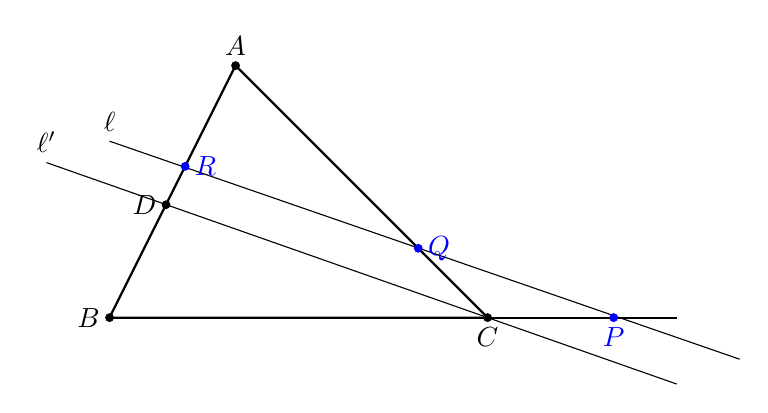
\begin{tikzpicture}[scale=1.6]
% Define the vertices
\coordinate (B) at (0,0);
\coordinate (C) at (3,0);
\coordinate (C') at (4.5,0);
\coordinate (A) at (1,2);
\coordinate (P) at (4,0);
\coordinate (P') at (5,-0.33);
\coordinate (Q) at (2.45, 0.55);
\coordinate (R) at (0.6,1.2);
\coordinate (R') at (0,1.4);
\coordinate (E) at (-0.5,1.23);
\coordinate (F) at (4.5,-0.527);
\coordinate (D) at (0.448,0.896);
% Draw the triangle
\draw[thick] (A)--(B)--(C)--cycle;
\draw[thick] (B)--(C');
% Draw medians
\draw[] (P')--(R') node[above] {$\ell$};
\draw[] (F)--(E) node[above] {$\ell '$};
% Mark the points
\fill (A) circle (1pt) node[above] {$A$};
\fill (B) circle (1pt) node[left] {$B$};
\fill (C) circle (1pt) node[below] {$C$};
\fill (D) circle (1pt) node[left] {$D$};
\fill[blue] (P) circle (1pt) node[below] {$P$};
\fill[blue] (Q) circle (1pt) node[right] {$Q$};
\fill[blue] (R) circle (1pt) node[right] {$R$};
\end{tikzpicture}
\end{center}
\[\frac{CQ}{QA} = \frac{RD}{AR} ,\quad  \frac{BP}{PC} =\frac{RB}{RD} .\]
\end{frame}

\begin{frame}{証明.}
	$ \displaystyle\frac{CQ}{QA} = \frac{RD}{AR} ,\quad  \frac{BP}{PC} =\frac{RB}{RD} $を使って,
\begin{center}
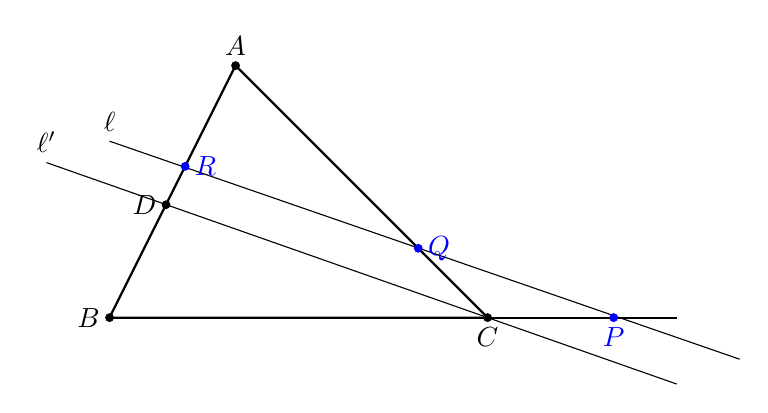
\begin{tikzpicture}[scale=1.6]
% Define the vertices
\coordinate (B) at (0,0);
\coordinate (C) at (3,0);
\coordinate (C') at (4.5,0);
\coordinate (A) at (1,2);
\coordinate (P) at (4,0);
\coordinate (P') at (5,-0.33);
\coordinate (Q) at (2.45, 0.55);
\coordinate (R) at (0.6,1.2);
\coordinate (R') at (0,1.4);
\coordinate (E) at (-0.5,1.23);
\coordinate (F) at (4.5,-0.527);
\coordinate (D) at (0.448,0.896);
% Draw the triangle
\draw[thick] (A)--(B)--(C)--cycle;
\draw[thick] (B)--(C');
% Draw medians
\draw[] (P')--(R') node[above] {$\ell$};
\draw[] (F)--(E) node[above] {$\ell '$};
% Mark the points
\fill (A) circle (1pt) node[above] {$A$};
\fill (B) circle (1pt) node[left] {$B$};
\fill (C) circle (1pt) node[below] {$C$};
\fill (D) circle (1pt) node[left] {$D$};
\fill[blue] (P) circle (1pt) node[below] {$P$};
\fill[blue] (Q) circle (1pt) node[right] {$Q$};
\fill[blue] (R) circle (1pt) node[right] {$R$};
\end{tikzpicture}
\end{center}
		\[\frac{AR}{RB}\cdot\frac{BP}{PC}\cdot\frac{CQ}{QA} =\frac{AR}{RB}\cdot\frac{RB}{RD}\cdot\frac{RD}{AR} = 1.\]
		\hfill \blacksquare
\end{frame}

\begin{frame}{直線$\ell$が\triangle ABC外にある場合.}
	\begin{center}
	\begin{tikzpicture}[scale=1.6]
  % Define the vertices
  \coordinate (B) at (0,0);
  \coordinate (C) at (3,0);
	\coordinate (C') at (6.5,0);
  \coordinate (A) at (1,2);
  \coordinate (A') at (1.5,3);
  \coordinate (A'') at (-0.5,3.5);
  \coordinate (P) at (6,0);
  \coordinate (P') at (6.5,-0.25);
  \coordinate (Q) at (0,3);
  \coordinate (R) at (1.2,2.4);
  \coordinate (R') at (-0.5,3.25);
  % Draw the triangle
  \draw[thick] (A)--(B)--(C)--cycle;
  \draw[] (B)--(C');
  \draw[] (A)--(A');
  \draw[] (A)--(A'');
  % Draw medians
	\draw[] (P')--(R') node[below] {$\ell$};
  % Mark the points
  \fill (A) circle (1pt) node[left] {$A$};
  \fill (B) circle (1pt) node[left] {$B$};
  \fill (C) circle (1pt) node[below] {$C$};
	\fill[blue] (P) circle (1pt) node[below] {$P$};
	\fill[blue] (Q) circle (1pt) node[right] {$Q$};
	\fill[blue] (R) circle (1pt) node[right] {$R$};
\end{tikzpicture}
\end{center}
\end{frame}

\begin{frame}{}
	\begin{center}
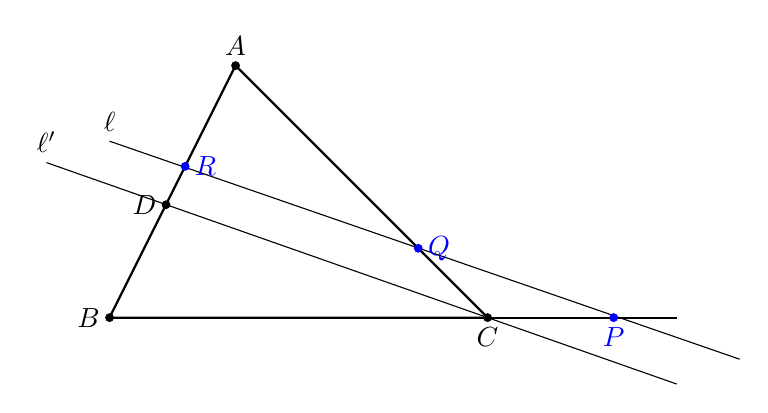
\begin{tikzpicture}[scale=1.6]
% Define the vertices
\coordinate (B) at (0,0);
\coordinate (C) at (3,0);
\coordinate (C') at (4.5,0);
\coordinate (A) at (1,2);
\coordinate (P) at (4,0);
\coordinate (P') at (5,-0.33);
\coordinate (Q) at (2.45, 0.55);
\coordinate (R) at (0.6,1.2);
\coordinate (R') at (0,1.4);
\coordinate (E) at (-0.5,1.23);
\coordinate (F) at (4.5,-0.527);
\coordinate (D) at (0.448,0.896);
% Draw the triangle
\draw[thick] (A)--(B)--(C)--cycle;
\draw[thick] (B)--(C');
% Draw medians
\draw[] (P')--(R') node[above] {$\ell$};
\draw[] (F)--(E) node[above] {$\ell '$};
% Mark the points
\fill (A) circle (1pt) node[above] {$A$};
\fill (B) circle (1pt) node[left] {$B$};
\fill (C) circle (1pt) node[below] {$C$};
\fill (D) circle (1pt) node[left] {$D$};
\fill[blue] (P) circle (1pt) node[below] {$P$};
\fill[blue] (Q) circle (1pt) node[right] {$Q$};
\fill[blue] (R) circle (1pt) node[right] {$R$};
\end{tikzpicture}
\end{center}
\end{frame}

\section{チェバの定理の逆 (Converse Ceva's theorem)}
\begin{frame}{}
  \begin{block}{チェバの定理の逆. (Converse Ceva's theorem)}
		\triangle ABCの各辺にある${\color{blue}P,Q,R}$が,
\[\frac{AR}{RB}\cdot\frac{BP}{PC}\cdot\frac{CQ}{QA} = 1.\]
を満たすとき,直線$AP,BQ,CR$は1点で交わる.
  \end{block}
	\begin{center}
	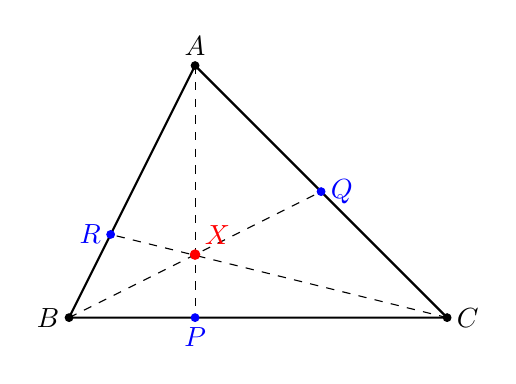
\begin{tikzpicture}[scale=1.6]
  % Define the vertices
  \coordinate (B) at (0,0);
  \coordinate (C) at (3,0);
  \coordinate (A) at (1,2);
  \coordinate (P) at (1,0);
  \coordinate (Q) at (2,1);
  \coordinate (R) at (0.33,0.66);
  % Draw the triangle
  \draw[thick] (A)--(B)--(C)--cycle;

  % Compute centroid G = (A+B+C)/3
  \coordinate (X) at (1,0.5);

  % Draw medians
  \draw[dashed] (A)--(P);
  \draw[dashed] (B)--(Q);
  \draw[dashed] (C)--(R);
  % Mark the points
  \fill (A) circle (1pt) node[above] {$A$};
  \fill (B) circle (1pt) node[left] {$B$};
  \fill (C) circle (1pt) node[right] {$C$};
	\fill[blue] (P) circle (1pt) node[below] {$P$};
	\fill[blue] (Q) circle (1pt) node[right] {$Q$};
	\fill[blue] (R) circle (1pt) node[left] {$R$};
  \fill[red] (X) circle (1.2pt) node[above right] {$X$};
\end{tikzpicture}
\end{center}
\end{frame}
\begin{frame}{}
	\begin{block}{応用例.}
		チェバの定理の逆を用いて,三角形の各頂点の内角の二等分線が1点で交わることを証明せよ.
	\end{block}
	\begin{center}
	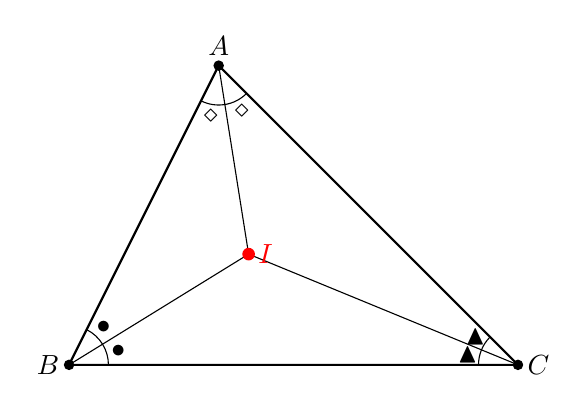
\begin{tikzpicture}[scale=1.9]
  % Define the vertices
  \coordinate (B) at (0,0);
  \coordinate (C) at (3,0);
  \coordinate (A) at (1,2);

  % Draw the triangle
  \draw[thick] (A)--(B)--(C)--cycle;

  % Compute centroid G = (A+B+C)/3
  \coordinate (I) at (1.2,0.74);
  \coordinate (L) at (1.2,0);
  \coordinate (N) at (0.54,1.08);
  \coordinate (M) at (1.73,1.27);
	 %\draw (I) circle (0.74);
  % Draw medians
  \draw[] (A)--(I);
  \draw[] (B)--(I);
	\draw[] (C)--(I);
%	\draw[dashed] (L)--(I);
%	\draw[dashed] (M)--(I);
%	\draw[dashed] (N)--(I);
  %\draw[dashed] (A)--(O);

%	\draw [line width=0.24pt] ($(L)!4pt!(C)$) -- ($(L)!4pt!(C)!4pt!90:(C)$) -- ($(L)!4pt!90:(C)$);
%	\draw [line width=0.24pt] ($(M)!4pt!(A)$) -- ($(M)!4pt!(A)!4pt!90:(A)$) -- ($(M)!4pt!90:(A)$);
%	\draw [line width=0.24pt] ($(N)!4pt!(B)$) -- ($(N)!4pt!(B)!4pt!90:(B)$) -- ($(N)!4pt!90:(B)$);

  % Mark the points
  \fill (A) circle (1pt) node[above] {$A$};
  \fill (B) circle (1pt) node[left] {$B$};
  \fill (C) circle (1pt) node[right] {$C$};
%  \fill (L) circle (1pt) node[below] {$L$};
%  \fill (M) circle (1pt) node[right] {$M$};
%  \fill (N) circle (1pt) node[left] {$N$};
  \fill[red] (I) circle (1.2pt) node[right] {$I$};

	 \path pic["$\bullet$",draw,angle radius=5mm,angle eccentricity=1.3] {angle = I--B--A};
	 \path pic["$\bullet$",draw,angle radius=5mm,angle eccentricity=1.3] {angle = C--B--I};
	 \path pic["$\diamond$",draw,angle radius=5mm,angle eccentricity=1.3] {angle = B--A--I};
	 \path pic["$\diamond$",draw,angle radius=5mm,angle eccentricity=1.3] {angle = I--A--C};
	 \path pic["$\blacktriangle$",draw,angle radius=5mm,angle eccentricity=1.3] {angle = A--C--I};
	 \path pic["$\blacktriangle$",draw,angle radius=5mm,angle eccentricity=1.3] {angle = I--C--B};
\end{tikzpicture}
\end{center}
\end{frame}

\section{メネラウスの定理の逆 (Converse Menelaus's theorem)}
\begin{frame}{}
  \begin{block}{メネラウスの定理の逆 (Converse Menelaus's theorem)}
		\triangle ABCの各辺を伸ばした直線上に,それぞれ${\color{blue} P,Q,R}$が,
		\[\frac{AR}{RB}\cdot\frac{BP}{PC}\cdot\frac{CQ}{QA} = 1.\]
		を満たすとき,3点${\color{blue} P,Q,R}$は一直線上に存在する.
  \end{block}
	\begin{center}
	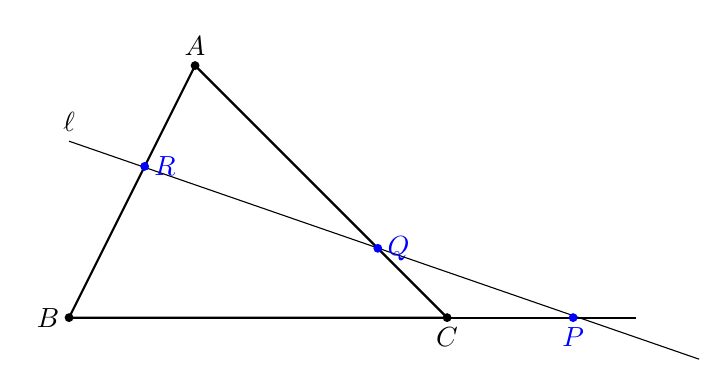
\begin{tikzpicture}[scale=1.6]
  % Define the vertices
  \coordinate (B) at (0,0);
  \coordinate (C) at (3,0);
	\coordinate (C') at (4.5,0);
  \coordinate (A) at (1,2);
  \coordinate (P) at (4,0);
  \coordinate (P') at (5,-0.33);
  \coordinate (Q) at (2.45, 0.55);
  \coordinate (R) at (0.6,1.2);
  \coordinate (R') at (0,1.4);
  % Draw the triangle
  \draw[thick] (A)--(B)--(C)--cycle;
  \draw[thick] (B)--(C');
  % Draw medians
	\draw[] (P')--(R') node[above] {$\ell$};
  % Mark the points
  \fill (A) circle (1pt) node[above] {$A$};
  \fill (B) circle (1pt) node[left] {$B$};
  \fill (C) circle (1pt) node[below] {$C$};
	\fill[blue] (P) circle (1pt) node[below] {$P$};
	\fill[blue] (Q) circle (1pt) node[right] {$Q$};
	\fill[blue] (R) circle (1pt) node[right] {$R$};
\end{tikzpicture}
\end{center}
\end{frame}

\end{document}
